\documentclass[conference]{IEEEtran}
\usepackage[pdftex]{graphicx}
%\usepackage{epstopdf}
\graphicspath{{./png/}{./eps/}}
\DeclareGraphicsExtensions{.pdf,.png}
\usepackage[caption=false,font=footnotesize]{subfig}
\hyphenation{op-tical net-works semi-conduc-tor}
\begin{document}
\title{The design and implementation of standards-based Grid single sign-on using federated identity}

\author{\IEEEauthorblockN{Weizhong Qiang, Aleksandr Konstantinov}
\IEEEauthorblockA{Department of Physics, University of Oslo}
}

\maketitle


\begin{abstract}
Security infrastructure is one of the most challenging tasks in the development, integration and
deployment of Grid middlewares. Even though the Grid community addresses the security issue 
through public key infrastructures (PKI) to support mutual authentication using X.509 certificates,
maintaining X.509 credentials is not that easy for non-IT-experts, and has proved to be an 
obstacle for a more wide deployment of Grid technologies. The identity federation 
is an increasingly popular technology that can facilitate cross-domain single sign-on
without requiring the users to maintain any credentials additional to their own institutional
accounts. We believe that utilizing identity federation for Grid middlewares is a promising path 
for the Grid technology to get more widely used.
This paper describes a single sign-on infrastructure developed as a part of the NorduGrid ARC Grid 
middleware. It adopts the identity federation standard (SAML), as well as Web Service approach. 
It focuses on a single sign-on solution at the middleware level for users to access Grids by only 
using their frequently used accounts, without being bothered to maintain X.509 credentials. 
Unlike other research which utilize identity federation on the Grid portal level, solution on
the middleware level can provide more flexibility.
In addition, the performance of single sign-on solution is measured. We identify performance limitations 
of security-related services inside this solution, and analyse the ways to avoid the limitations.
To our knowledge, the work presented in this paper is the first evaluated implementation that utilizes 
identity federation for Grid usage on the middleware level.
\end{abstract}

%-------------------------------------------------------------------------
\section{Introduction}
\label{sec:intro}
Grid infrastructures facilitate interoperability between wide-scale, cross-domain heterogeneous 
resources, as well as the user access to these resources. In terms of security issues, a Grid security 
infrastructure should provide as simple accessibility as possible without loosing the security benefits.

Many current Grid communities predominantly use the Grid Security Infrastructure (GSI)~\cite{IFoster98} as the \textit{de facto} 
standard for authentication and transport level security. It builds on the Public Key Infrastructure
(PKI) to support authentication using X.509 certificates. GSI-based Grid deployment requires mutual authentication.
Mutual authentication means that Grid users have to possess X.509 
credentials. To obtain an X.509 credential, a user needs to contact a designated Registration Authority (RA)
which will check the user's personal data and eventually approve her certificate request; afterwards,
the respective Certificate Authority (CA) can issue the certificate following the approval from 
the RA. The whole process is arduous and may take quite some time.
Meanwhile, to maintain an X.509 certificate is also not so easy for the non-IT-skilled community to deal 
with, since users have to periodically create proxy certificates by using Grid-specific command line 
utilities, such as \texttt{grid-proxy-init} or \texttt{voms-proxy-init}. Also, operating CAs or RAs is not an  
easy task, especially when the community of Grid users is getting much larger.

On the other hand, users normally would already have some frequently-used campus or company 
accounts/credentials such as username/password. We believe that enabling Grid users to use their institutional 
credentials rather than the X.509 certificate to access Grids is a promising way 
to make the Grids more easily accessible, as well as to extend the user community of Grids
to a much larger scale.

To enable users to utilize the institutional credentials to access Grid, some issues need to be 
addressed. Firstly, the Grid middleware needs to be extended to support the authentication based on
institutional credentials instead of X.509 certificates; secondly, in order to interoperate with
those Grid infrastructures which require X.509 certificate-based mutual authentication, an approach
should be provided for obtaining X.509 certificate based on the institutional credentials; thirdly,
the single sign-on characteristic should be provided so that users can authenticate once and then traverse 
from Grid resources to Grid resources without being prompted to authenticate again at each resource.

The new approach in the ARC~\cite{MEllert07} Grid middleware is to utilize the identity federation 
standards, specifically, the Security Assertion Mark-up Language (SAML) specification, and Web 
Service standards, to facilitate the Grid single sign-on.

The rest of this paper is organized as follows: Section~\ref{sec:arcmiddleware} presents the 
ARC Grid middleware, and in particular its new architecture. Section~\ref{sec:intergrationSAML2SSO} 
describes the solution of using federated identity for 
Grid authentication by using \texttt{SAML2 Web Browser SSO Profile (SAML2SSO)} profile; 
Section~\ref{sec:fedidtoX509} describes
how to obtain X.509 credentials based on federated identity, and how to use such for 
accessing multiple Grid resources; Section~\ref{sec:perfeval} is dedicated to performance evaluation;
Section~\ref{sec:relatedwork} describes the related work; Section~\ref{sec:conclusion} 
contains conclusions and future work outlook.

%-------------------------------------------------------------------------
\section{ARC Grid middleware}
\label{sec:arcmiddleware}

ARC (Advanced Resource Connector)~\cite{MEllert07} is an open source Grid middleware solution released 
under Apache license. ARC middleware aims at developing self-organized, 
fault-tolerant, non-intrusive, easy-manageable Grid middleware. 
The current production version of ARC provides Grid services for job submission and 
management, resource characterization, resource aggregation and discovery, basic data 
management, integration of Grid security solution, and so on. It has been 
deployed and used in production environment, and is one of the most widely deployed Grid
solutions in Europe.

Further development of new ARC components is pursued by the EU KnowARC project~\cite{KnowARClink}, 
based on the functionality of the current production ARC middleware. It aims at 
implementing a Web Service oriented Grid middleware which will provide higher levels of 
resource and user abstraction through a well-defined Web Service interface~\cite{KnowARCDesignlink} 
in order to provide interoperability with other Web Service oriented Grid middlewares, as well as 
other Web Service compatible applications.

The key part of the new approach is a lightweight Web 
Service container called Hosting Environment Daemon (HED), which provides hosting environment 
for various services at application level, as well as a number of modules to support flexible, 
interoperable, and efficient communication mechanism for building SOAP-based Web Services. 
The design of the HED is built around the idea of flexibility and modularity,
such that the application service developers can simply concentrate on the application 
level Web Service implementation by only using the core minimum amount of components. It 
also simplifies work on the middleware level: for example, it makes possible to implement another 
communication protocol or authentication mechanism. Meanwhile, a service administrator can easily 
configure and deploy the middleware and application for different kinds of requirements 
without having to know much about the implementation. 

The architecture of HED is illustrated in Figure~\ref{fig:HED}. In general, there 
are several components called Message Chain Component (MCC) which are in charge of implementing 
different protocol levels. For example, as shown in the message flow, the HTTP MCC 
will process a stream from the TLS MCC to parse the HTTP message and pass its body to the SOAP 
MCC, and also process the SOAP response from the SOAP MCC to generate the HTTP message 
for the TLS MCC.

Dotted line in Figure~\ref{fig:HED} shows an alternative path for the information 
to propagate among MCCs. A service administrator can configure the MCCs according to the 
interoperability requirements with a counterpart. For instance, the configuration marked 
with the dotted line is compatible with the WSE (Web Services Enhancement for .NET) SOAP 
message mechanism (c.f. WSE SoapSender and SoapReceiver)~\cite{WSElink}. Another configuration 
could be SOAP over HTTPG (HTTP over GSI) which is needed to interoperate with services 
like the Storage Resource Manager (SRM)~\cite{A.Shoshan03} service. This shows the 
flexibility of HED in terms of protocols support.

\begin{figure}
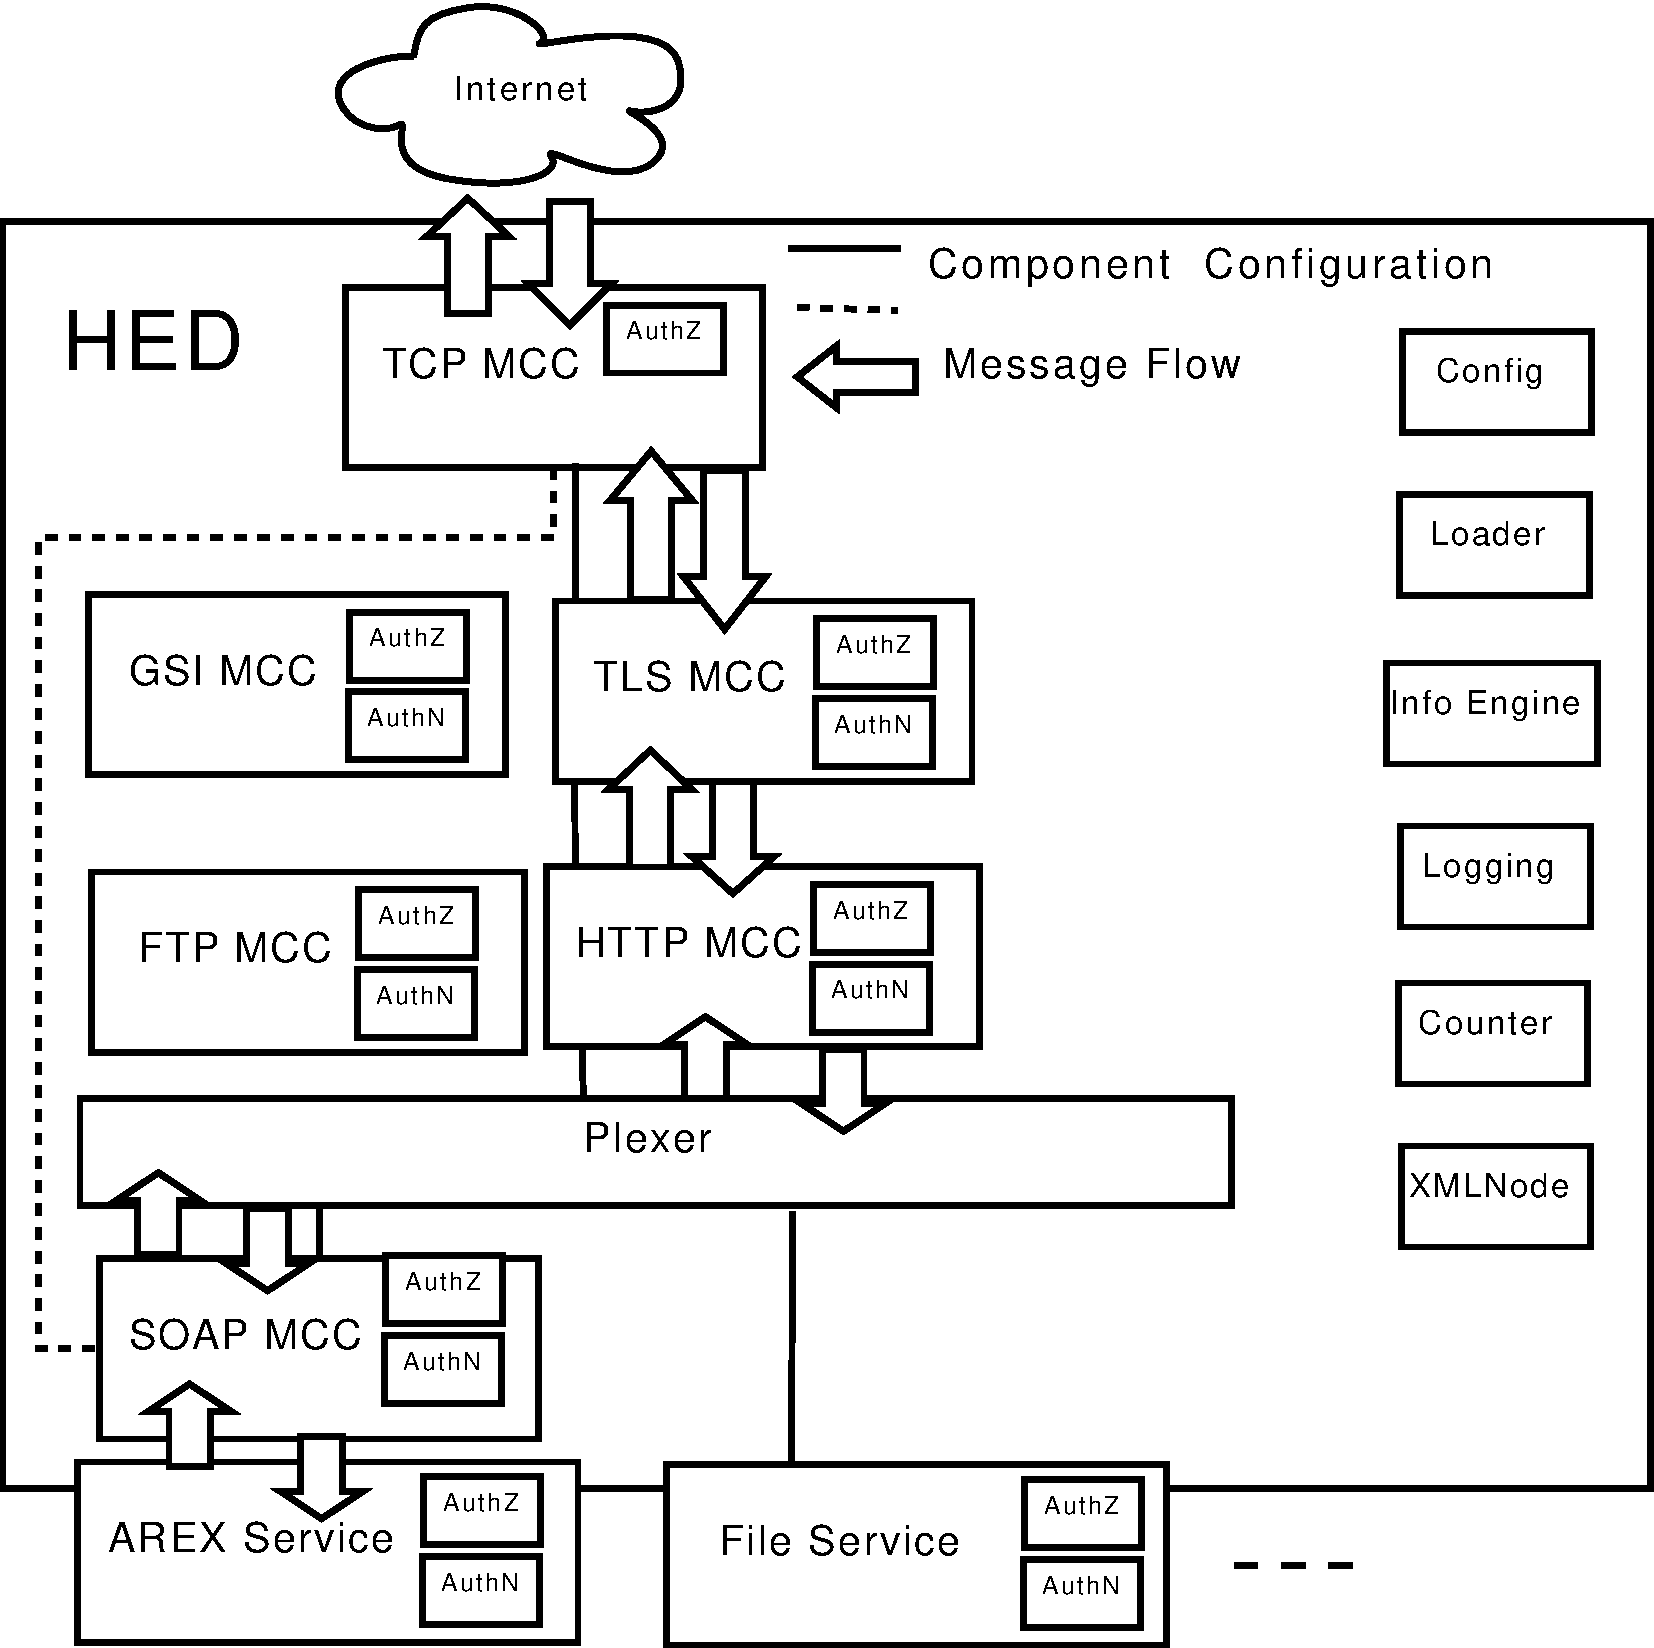
\includegraphics[width=0.9\columnwidth]{HED.pdf}
\caption{The example of Host Environment Daemon deployed with A-REX and File services}
\label{fig:HED}
\end{figure}

HED contains a flexible security framework for implementing and enforcing
security-related functionality, such as authentication and authorization. 
Each security-related functionality can be implemented as a pluggable and
configurable component (plug-in) called \textit{SecHandler}. Each MCC or Service is usually
configured with two queues of SecHandler -- one for incoming messages and one for
outgoing messages, respectively. In Figure~\ref{fig:HED}, the ``AuthZ'' and ``AuthN'' sub-modules
inside MCCs and Services are examples of SecHandler.

%-------------------------------------------------------------------------
\section{Grid authentication using federated identity: Integrating SAML2SSO
profile}
\label{sec:intergrationSAML2SSO}
Identity federation is an emerging technology which enables the identity
information to be trustily transferred across autonomous security domains. By using identity
federation, users from one domain can access another domain without the need for a direct trust
relationship between users and accessed domains, i.e., users can use accounts from their host
domains to access external domains, and accessed domain does not need to maintain accounts
for those external users. Identity federation does not enforce specific authentication
mechanisms, therefore various types of authentication can be supported
between users and their host domains, and users are able to use their frequently used accounts or credentials to
accomplish authentication. Considering Grid use cases, we see that utilizing an existing account to
access Grid without being bothered to apply for and manipulate a X.509 credential
would be attractive for Grid users.

Shibboleth~\cite{Shiblink} is the one of the several implementations of the
identity federation, which is based on the OASIS Security Assertion Markup Language (SAML) 2.0
specifications~\cite{SAMLlink}. In terms of authentication, Shibboleth implements SAML2.0 web browser SSO
profile~\cite{SAMLprofiles}, which  defines two functional components, an Identity Provider and a Service Provider. The
Identity Provider (IdP) is responsible for creating, maintaining, and managing user identity,
while the Service Provider (SP) is responsible for controlling access to services and resources by
analysing the SAML assertions produced and issued by the IdP upon request (request from
client application to the service/resource that is protected by SP).

In the implementation of ARC middleware, SAML2.0 web browser SSO profile is
supported by implementing the functionality of service provider and web browser's user agent,
and utilizing Shibboleth IdP implementation for the functionality of identity provider. The
user agent functionality is for mimicking the behaviour of web browser's user agent for
authentication, such as the HTTP redirection and the HTTP cookie processing. Implementation
of the user agent is based on the the HTTPS client interface of ARC, since the client
interface of ARC can support different protocols which are incarnated by different MCCs.

\begin{figure}
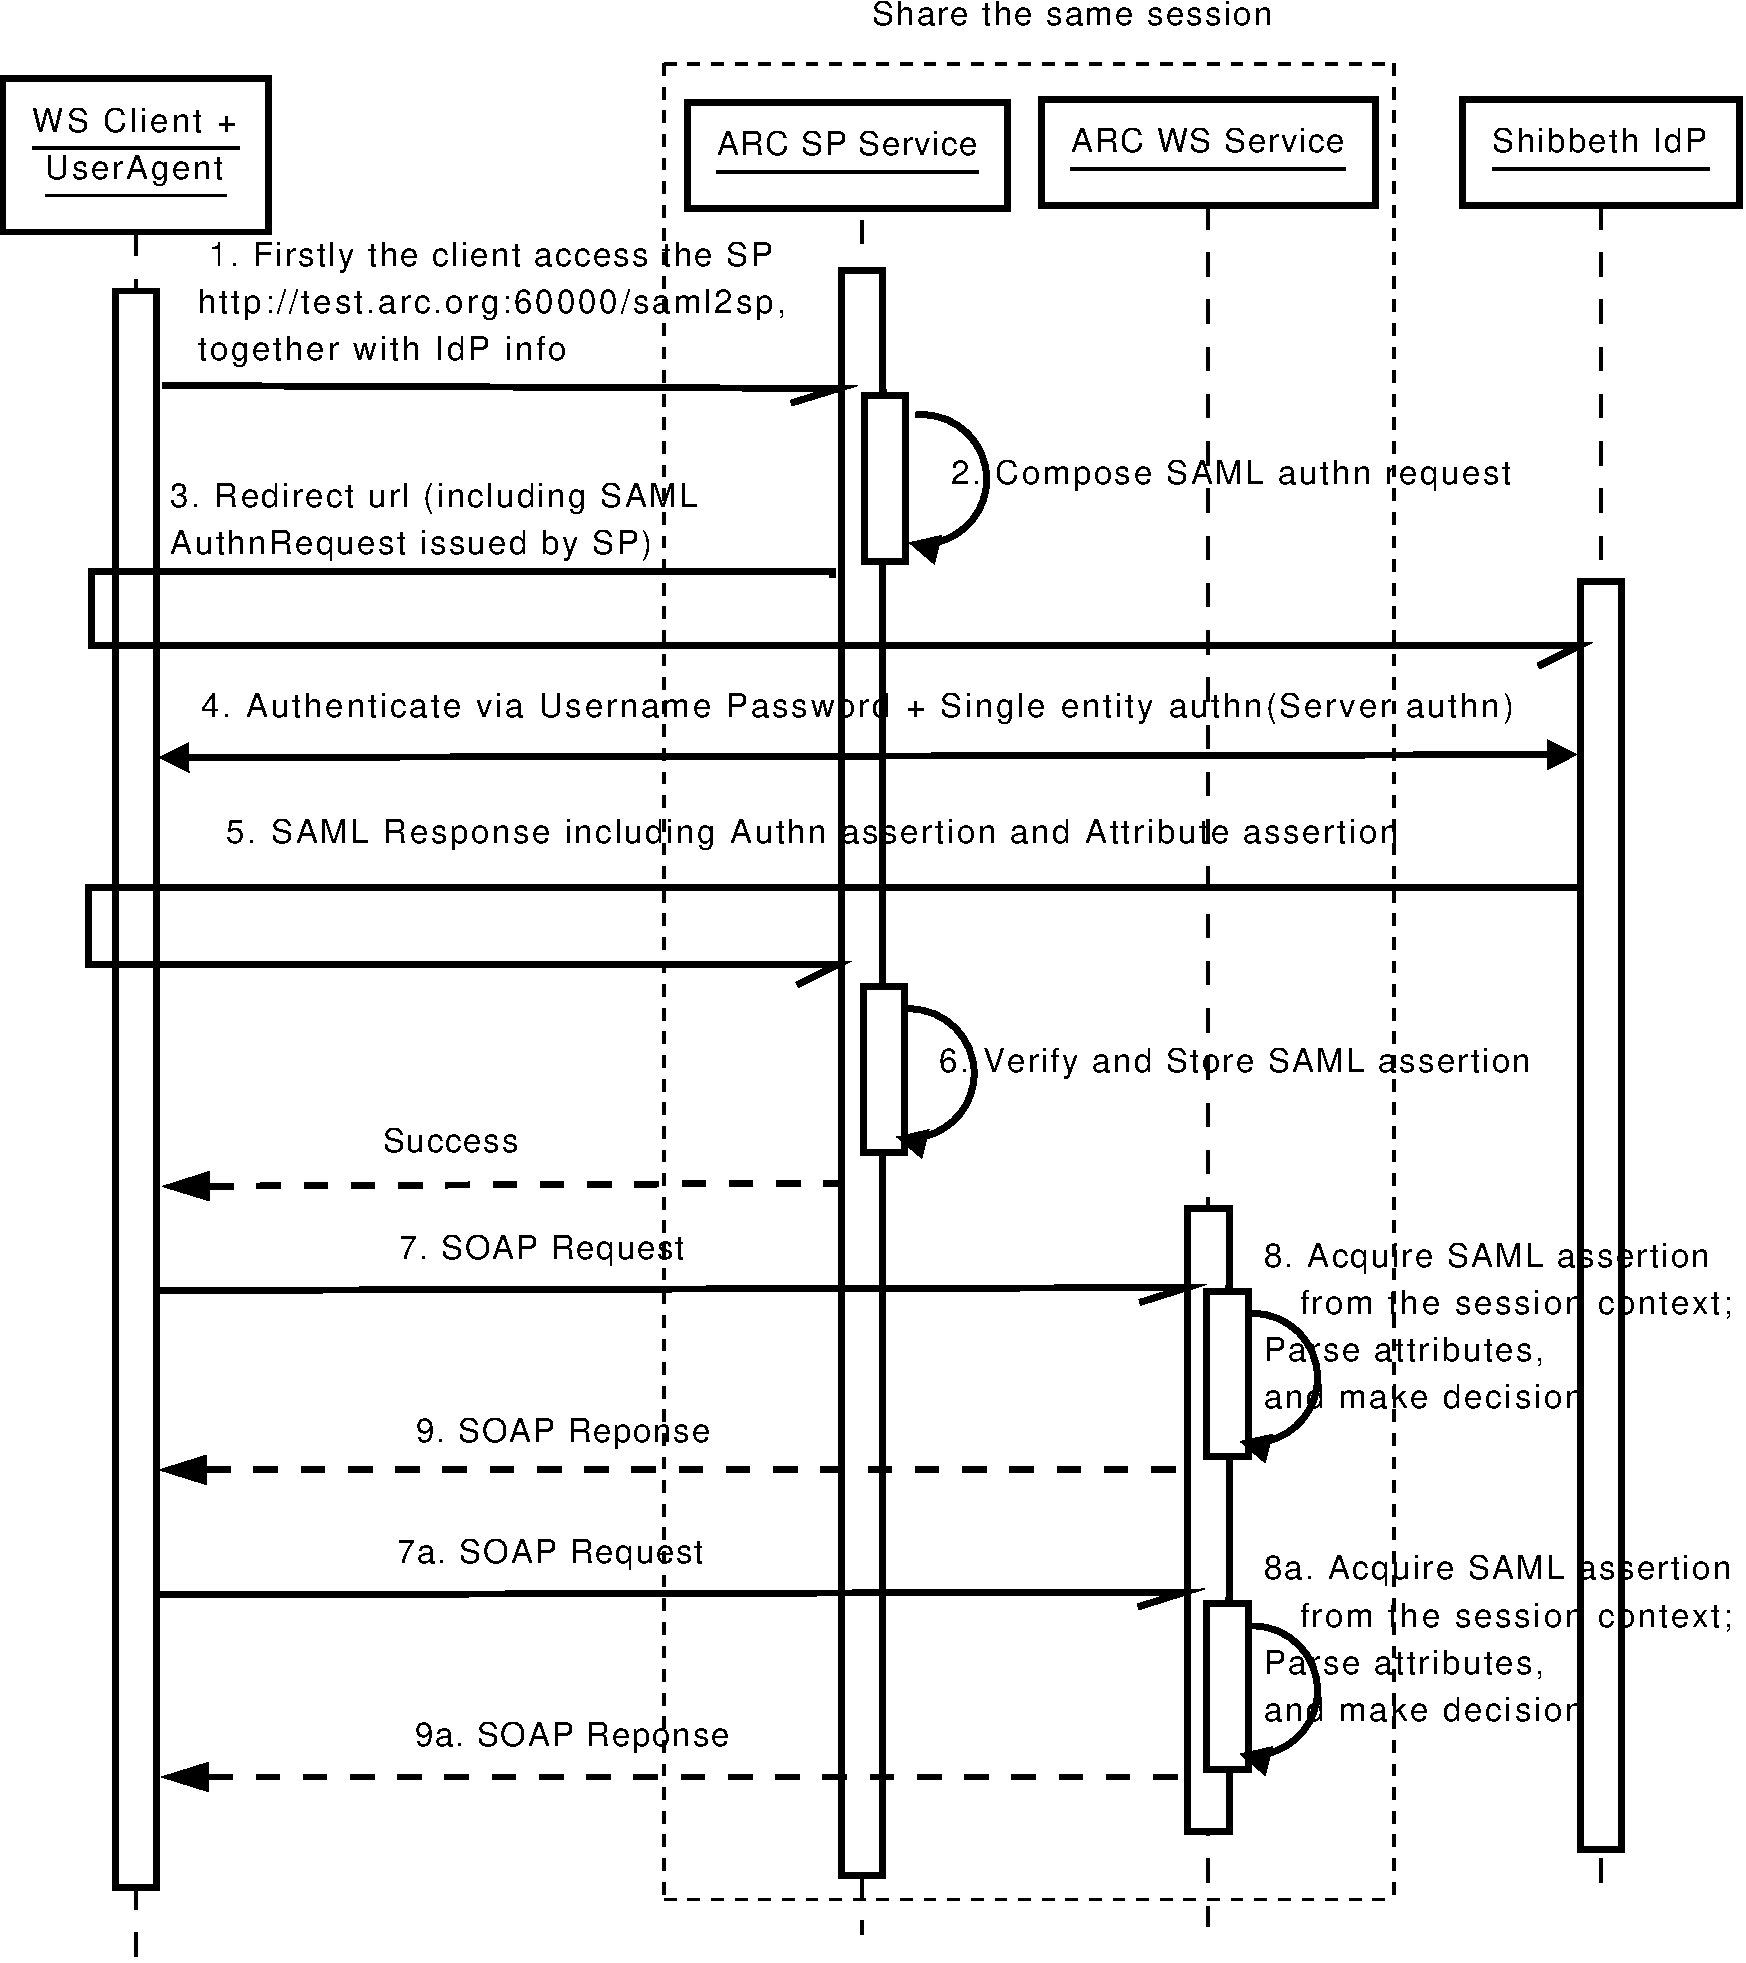
\includegraphics[width=1.0\columnwidth]{SAML2SSO_UML.pdf}
\caption{Sequence diagram of the integration of SAML2.0 SSO profile in SOAP invocation 
between ARC WS Client and Web Service}
\label{fig:SAML2SSOUML}
\end{figure}

Figure~\ref{fig:SAML2SSOUML} shows how the SAML2.0 SSO profile is integrated
into the SOAP invocation between ARC WS Client and Web Service. Steps 1 to 5 in
Figure~\ref{fig:SAML2SSOUML} are similar to those steps depicted in the SAML2 Web Browser SSO profile, with
the difference that we specify the way how does the service provider determine which identity
provider to use (identity provider discovery) by enabling the client to send the IdP name to the service
provider. We also specify the way how does the client (user agent)
authenticate against a service provider by implementing the form-based HTTP authentication which uses username and
password for authentication between the user agent and a service provider (rather than the X.509 client authentication),
which is compatible with the Username/Password login handler of the Shibboleth IdP.

In step 6, the service provider (SP Service) verifies and checks the SAML
response, decrypts and stores the SAML assertion into session/connection context. That assertion includes the
AuthnStatement and AttributeStatement elements. From step 8 to step 10, the WS client first
launches the SOAP invocation via the same connection as the one which is used by the user agent to contact an SP
Service, and then the Grid/Web Service checks the AuthnStatement stored in the session context to see whether the
AuthnStatement is valid or expired. If valid, the service handles the SOAP request and returns the SOAP response to
the WS client. Note that the ``connection'' and ``session'' are interchangeably used in this paper, with
the same meaning for a TCP connection.

Note also that in the current implementation the service requires the WS client
to re-use the same TCP connection as the one used by the user agent in step 5, in order to
guarantee that the validity of the SAML2SSO result is applicable to the SOAP invocation process. On the service
side, the session re-using is accomplished by deploying the SP service and other
functional Grid/Web Service(s) together in the same service container.

There are a several benefits with integrating the SAML2.0 SSO profile for
Grid/Web service authentication. Firstly, the client certificate authentication can be switched off, so that
users would not need to apply and maintain X.509 credentials. Secondly, some implementations of
identity provider, such as Shibboleth IdP, can cache the authentication result through session management
once the user has succeeded to authenticate, and for a short period this authentication result
is valid, so that the next time the user authenticates against IdP, the user agent can just feed
IdP with the last successfully authenticated session's identity rather than feed IdP with
the username and password again. So the user (or the client on behalf of that user) can access multiple
security domains by only providing his name and password once, which is also a characteristic of
single sign-on. Lastly, even though there are several implementations of identity providers,
most of them are standard-compliant, so the solution implemented in ARC middleware can
interoperate with other identity provider implementations with minimum change.

%-------------------------------------------------------------------------
\section{Bridging federated identity and X.509 credential}
\label{sec:fedidtoX509}
The integration of SAML2SSO profile in Section~\ref{sec:intergrationSAML2SSO}
provides complete single sign-on in the Grid middleware level without requiring X.509
certificate on the client side.

However, many widely used Grid middlewares are based on GSI which requires mutual X.509
authentication. Meanwhile, Web Service based Grid applications mostly require client
certificate authentication. To bridge the gap between federated identities and X.509 credentials, a short
lived credential service (SLCS) is implemented through which a user can get a short-lived X.509
certificate only by providing his username and password and authenticating through the SAML2SSO
profile.

Also, in order to provide single sign-on capability for services that act on
behalf of the user to invoke other services, a X.509 credential delegation service is implemented,
which is based on SOAP communication rather than the proprietary GSI communication which is used
in the delegation services such as MyProxy~\cite{myproxy}.

\subsection{Short-lived credential service}
\label{sec:slcs}
The sequence diagram of a SLCS process is the same as the diagram shown in 
Figure~\ref{fig:SAML2SSOUML}, with the SOAP request (the message of step 8 of 
Figure~\ref{fig:SAML2SSOUML}) including an X.509 request, and the SOAP response (the message of step 10 
of Figure~\ref{fig:SAML2SSOUML}) including an X.509 certificate and a CA certificate that is used 
to sign this X.509 certificate. In detail, the SLCS client firstly accomplishes the SAML2SSO profile, 
then sends the SOAP request to the SLCS service with the X.509 request embedded. The SLCS
service makes access control decision according to the SAML assertion stored in the session
context, and issues a certificate (with 12 hours lifetime) with SAML attributes as the X.509
certificate extension. The SLCS client then gets the SOAP response with the X.509
certificate and the CA certificate embedded.

Since the lifetime of the short lived credential is short, it is
permissible to protect the private key by using the local file system permissions instead of encrypting
it by using a pass-phrase. Therefore, no manual interactivity is required to encrypt
the private key. Hence a single sign-on is provided, since the user only needs to enter his
password when starting a SAML2SSO profile.

A critical issue for the SLCS service is how to compose a distinguished name
(DN) for the certificate. Since the ``eduPersonPrincipalName'' (see eduPerson schema~\cite{eduSchemalink})
is identical to the user that accomplishes SAML2SSO profile, we pick up
``eduPersonPrincipalName'' from SAML attributes that returned from Shibboleth IdP, and use it to compose
the DN. A typical example of the eduPersonPrincipalName 
could be \textit{alice@example.org}. In such a case the composed DN would be,
for example,\\``/O=knowarc/OU=example.org/CN=alice''.

By using the SLCS service, a user can easily access Grid services that
require X.509 credentials on the client side from anywhere, simply by running the SLCS
client command and providing his username and password.

\subsection{X.509 credential delegation service}
\label{sec:creddeleg}

\begin{figure}
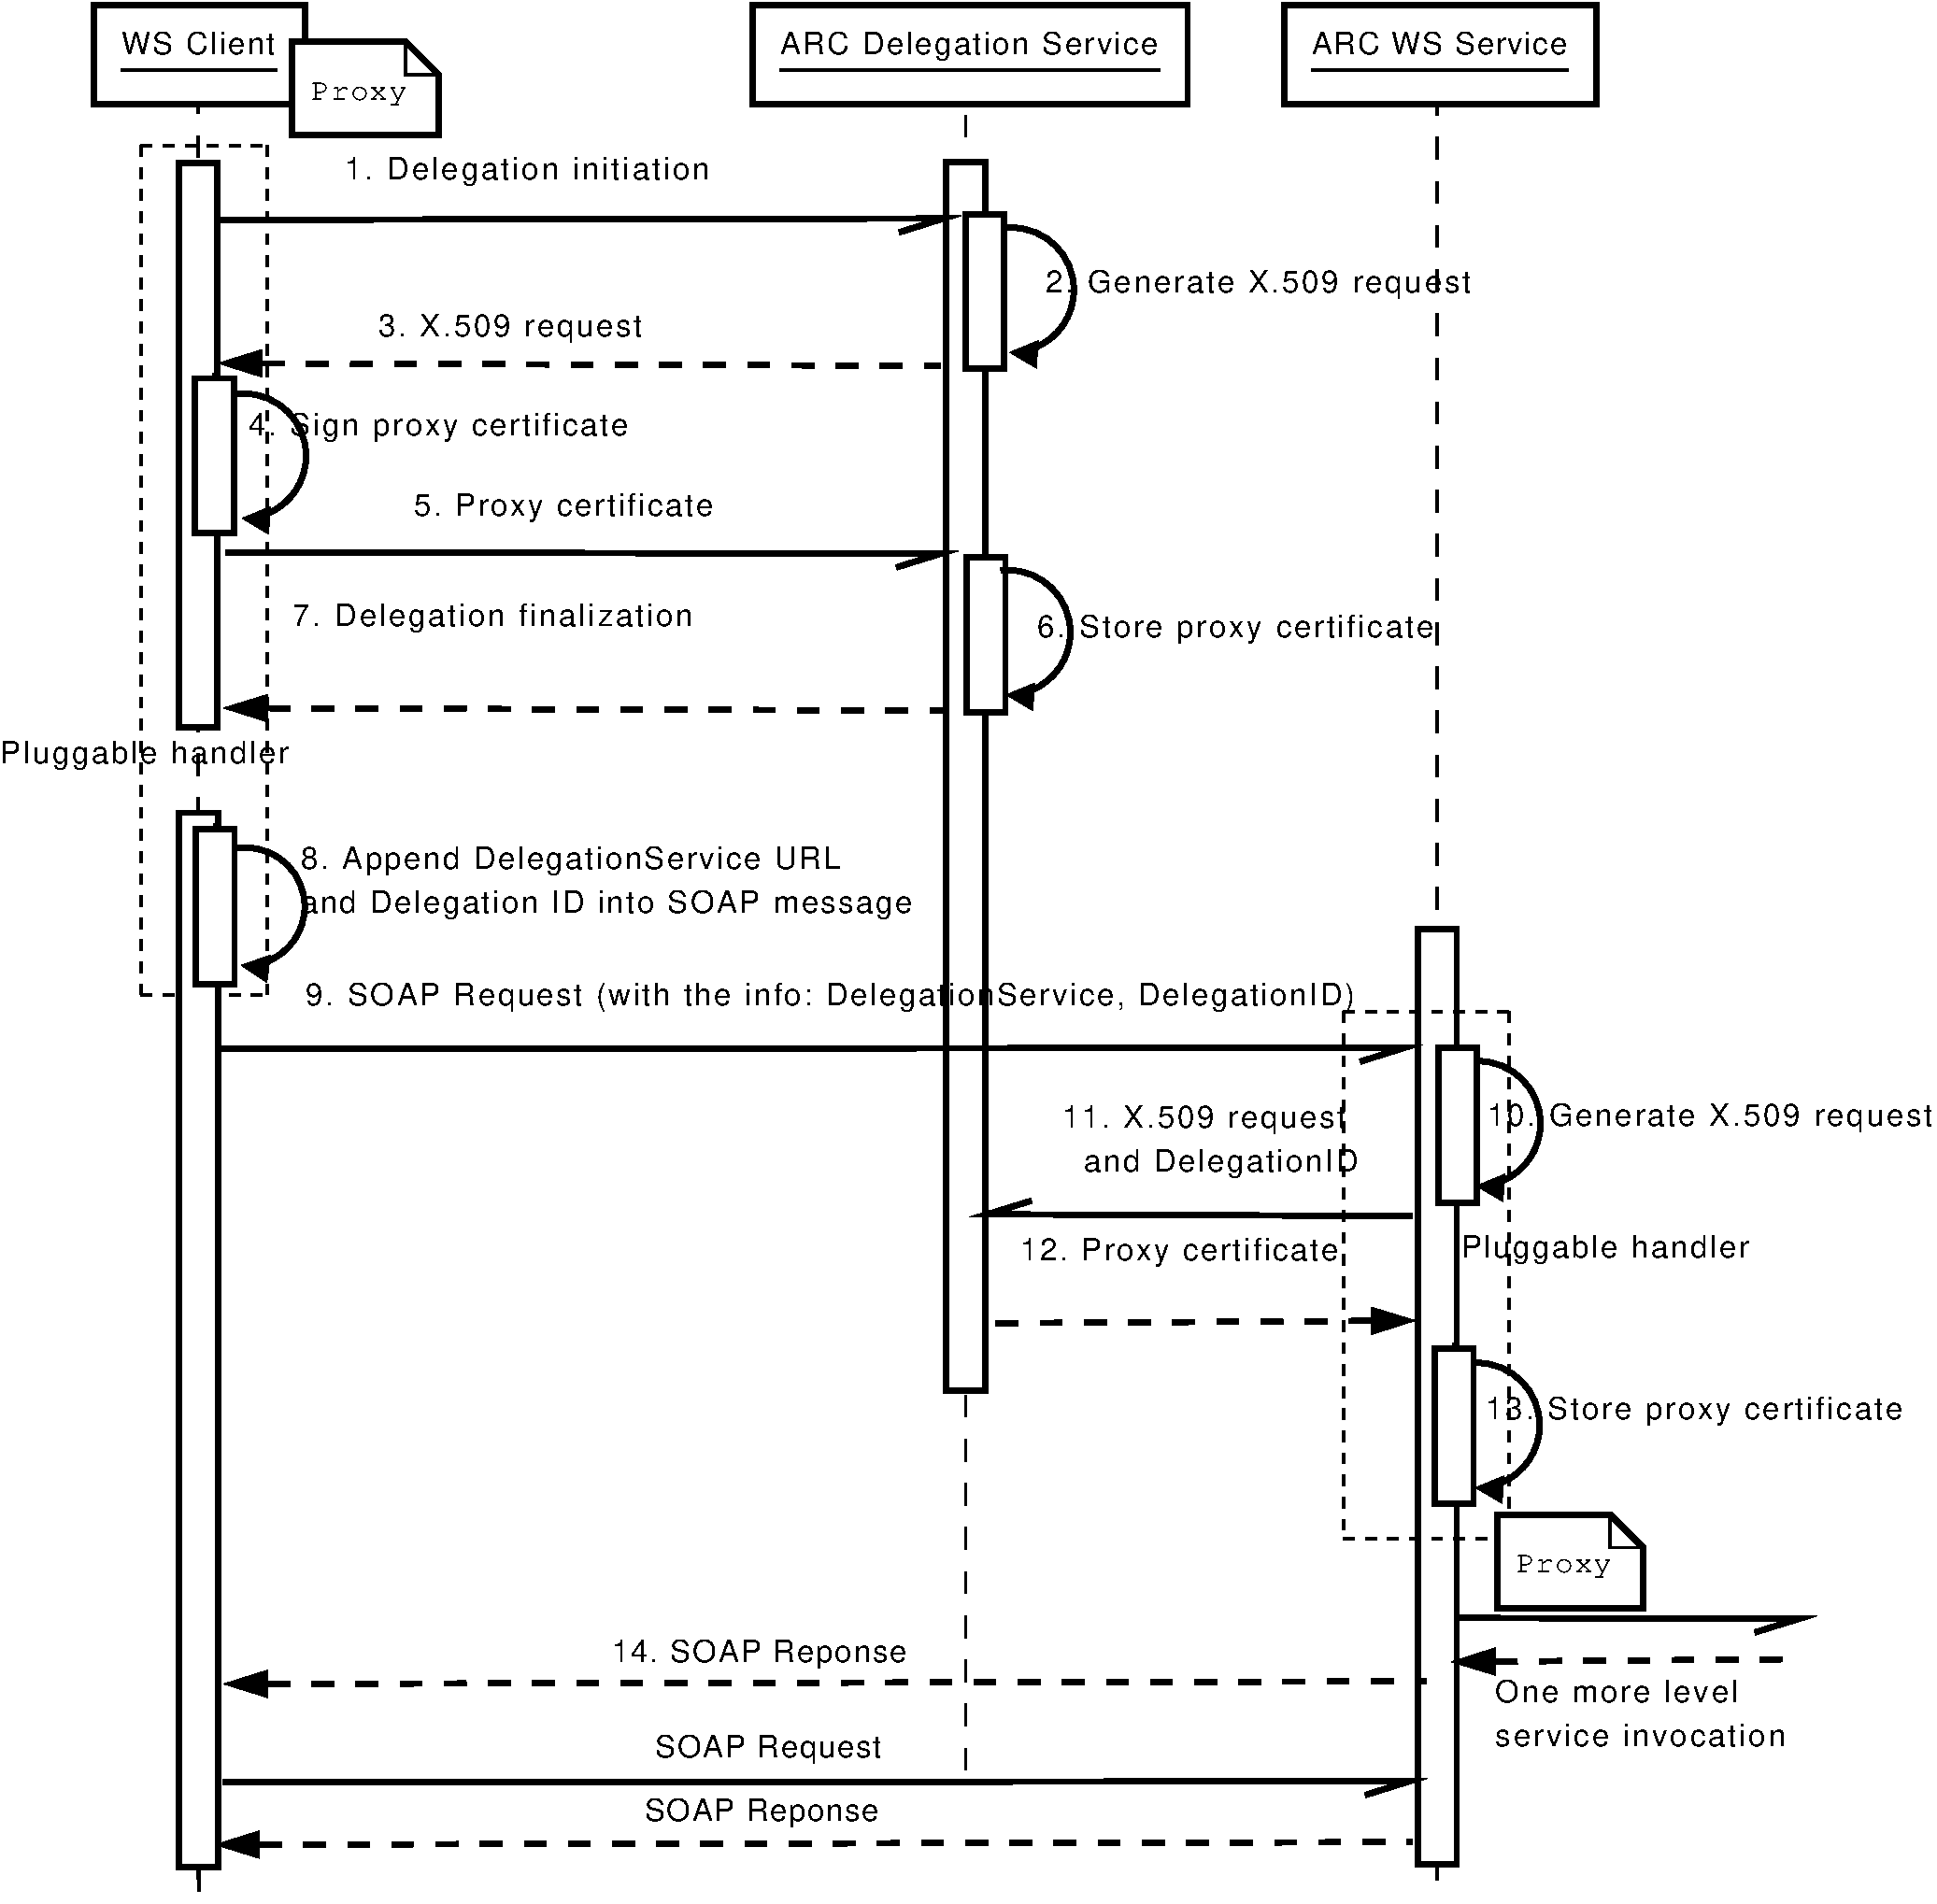
\includegraphics[width=1.0\columnwidth]{Delegation_UML.pdf}
\caption{Sequence diagram of the usage of delegation service in SOAP invocation 
between ARC WS Client and Web Service}
\label{fig:DelegUML}
\end{figure}

The delegation service usage sequence diagram is shown in
Figure~\ref{fig:DelegUML}. Firstly, the client needs to delegate
the proxy certificate or the short-lived certificate to a delegation service
through steps 1 to 7.
Then this client invokes the peer Web Service by appending the delegation
information (URL of delegation service and the delegation ID corresponding to the above delegation) to the
SOAP body. The Web Service then sends a X.509 request and the delegation ID to the delegation
service which is specified by the client side, and gets back a delegated certificate
which can be composed together with the private key for a proxy certificate. The Web Service could use this
proxy certificate to represent the user to invoke another Web Service, which either could cause
one more process of delegation (steps 1 to 13) if another delegation service is specified, or
could directly start from step 8 if the same delegation service is specified as the one in the
previous delegation process.

The client only needs to delegate the certificate to the delegation service once
per session; it does not have to do delegation for subsequent SOAP invocations after the first one.

The functionalities of both client and service sides are implemented as
pluggable handlers which can be configured into the client and service configuration, so that the service or
client implementation itself does not need to be changed.

We assume that the short-lived certificate is used by the client, so that the
SLCS service together with the delegation service can provide single sign-on from user's federated
identity, while keeping the interoperability to those Grid/Web services that require mutual authentication
using certificate.

%-------------------------------------------------------------------------
\section{Performance Evaluation}
\label{sec:perfeval}
The following sections evaluate the performance of the HED versus Axis2/C, as 
well as the performance related to the integration of SAML2SSO profile, 
short-lived credential service, and delegation service.

\subsection{Performance comparison between HED and Axis2/C}
\label{sec:perhedandaxis}
Since the implementation of HED includes an alternative SOAP implementation
which is the base of the security related web services described in this paper, it is useful to
compare the performance of HED and other SOAP implementations. Here we compare 
the performance of HED and Axis2/C (v1.5.0), because we need to demostrate that the performance of HED
is at least comparable to other implementations. We do not compare the performance of HED 
with other SOAP implementations such as AxisJava, gSOAP, XSOAP4, etc., because a complete 
performance comparison between HED and all the other SOAP implementations is not the main 
goal of this paper to achieve, and a partial performance comparison is enough. Another reason
of choosing Axis2/C is because it is also implemented in C/C++ programming language.

For the service side, we implement two simple ``echoString'' services in HED and
Axis2/C. The ``echoString'' provides a simple SOAP portType which will output the same value
as it gets from input. For the client side, we develop a client by using the client API of ARC, to
invoke ``echoString'' services from Axis2/C and HED. Service invocation just sends a short
string to a service, and gets back the same string. One test involves a set of clients
which run simultaneously. Each client runs for a fixed period of time, and invokes the service as many
times as it can during the test period. Multiple clients are launched by creating multiple threads in
one test. Two values are measured: average response time and throughput. Average response
time is computed by counting the average value of the response time for each invocation.
Throughput is computed by counting number of invocations per second or per minute.

The two ``echoString'' services run in a test machine equipped with a 3GHz Intel
Pentium dual-core CPU and 2GB memory, Red Hat Enterprise Linux 5. The client runs in another
machine equipped with 2.0GHz AMD Athlon CPU and 1GB memory, Red Hat Enterprise Linux 5. The
Axis2/C service is run using the httpd module on Apache Http Server version 2.2.11 instance. 
We use all the default configurations in the Apache Http Server, and complie Axis2/C
with default options except specifying the ``--with-apache2'' option.

\begin{figure}
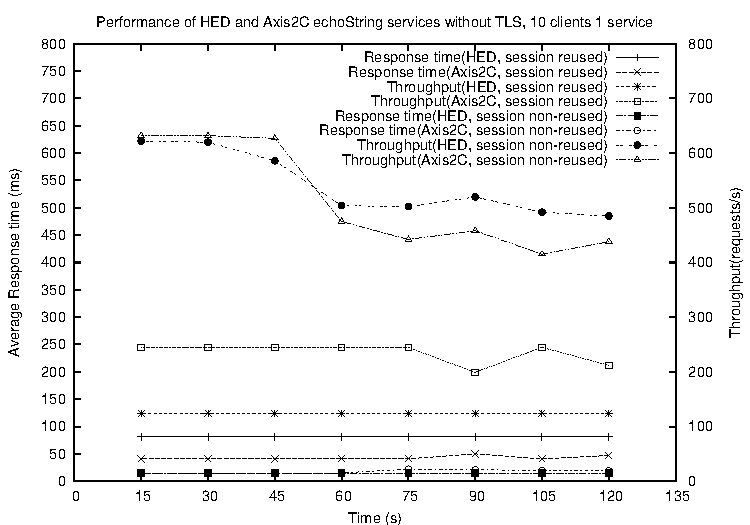
\includegraphics[width=0.9\columnwidth]{HED2Axis_thread10.pdf}
\caption{Performance results for HED and Axis2C: 1 service and 10 clients}
\label{fig:HED2Axis_thread10}
\end{figure}

\begin{figure}
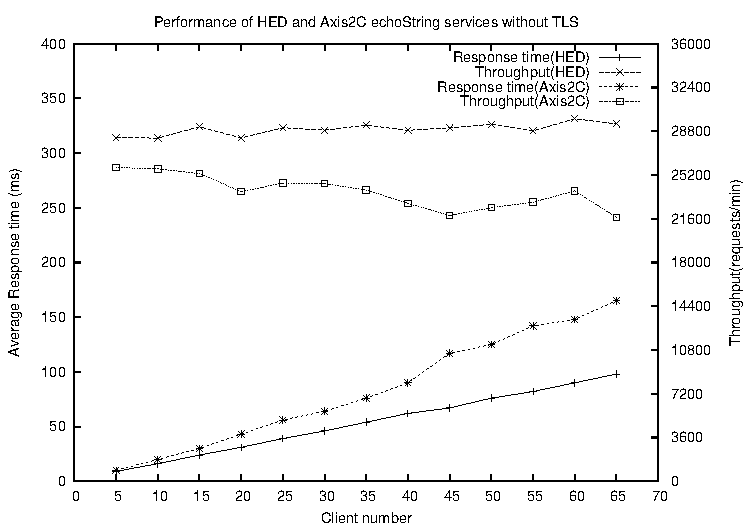
\includegraphics[width=0.9\columnwidth]{TCP_thread_all.pdf}
\caption{Performance of HED and Axis2C echoString services without TLS:
performance
changes with client numbers; session not re-used }
\label{fig:TCP_thread_all}
\end{figure}

\begin{figure}
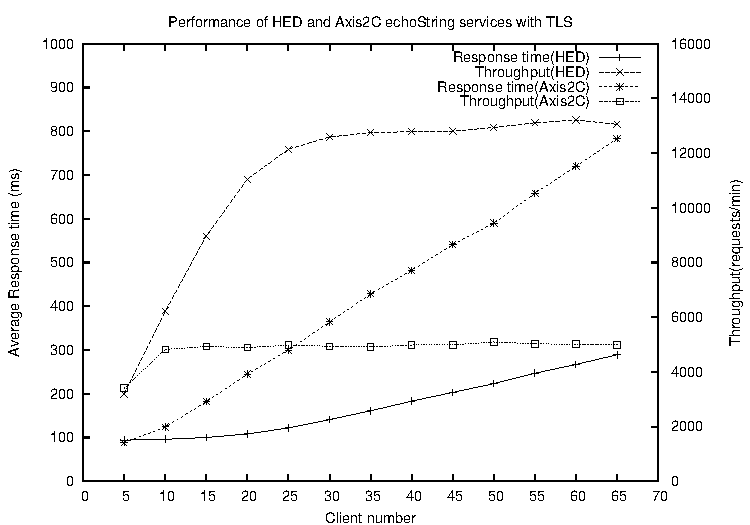
\includegraphics[width=0.9\columnwidth]{TLS_thread_all.pdf}
\caption{Performance of HED and Axis2C echoString services with TLS: performance
changes with client numbers; session not re-used}
\label{fig:TLS_thread_all}
\end{figure}

Figure~\ref{fig:HED2Axis_thread10} shows results of performance comparison with
ten clients being launched.
Two types of experiments are shown: session re-used and session not re-used.
``Session re-used'' means that all the SOAP invocations on each client share
the same session (TCP connection); while ``Session not re-used'' means that each invocation
launches a new session.

For the ``Session re-used'' experiments, we see that the average response time
in HED is about 81ms which is twice the value for Axis2/C, and the throughput in HED is about half
of the value for Axis2/C. One observation is that the performance results of HED are quite stable, with
the average response time and throughput almost unchanged for different time points.
For the ``Session not re-used'' experiments, the average response time in HED is
almost the same as the value for Axis2/C, with the value 15ms. On the other hand, the throughput in
HED is close to the value for Axis2/C. 

Since the echoString service is a simple service which occupies little
resources and has stable time for the processing service logic itself, and also since the experiments are done over the local
network, we can speculate that the response time shown in Figure~\ref{fig:HED2Axis_thread10} mainly
corresponds to the processing time in the container itself.
With the stability characteristic of the performance, we can speculate that the
service container itself will have a stable impact on the performance of other services.

To compare more deeply performance of the services in HED and Axis2/C, some
tests have been done to investigate how does the number of simultaneous clients affect
the performance. Figure~\ref{fig:TCP_thread_all} shows performance results for echoString
services with the changing number of clients. In this set of experiments, the session is not re-used, and secure
communication is not used. Each experiment is executed for a relatively long duration (two minutes),
so that there are enough instances of service invocation and thus the performance measurements are
reliable. We see that the response time of services in both HED and Axis2/C starts from a
similar value (when the client number is five) and changes linearly with the number of
clients, while the service in HED provides shorter response time with the value being around two thirds of the
response time of the service in Axis2/C when the number of clients becomes higher.
In the case of throughput, the service in HED provides stable throughput, while
the service in Axis2/C provides throughput which  becomes slightly smaller when number of clients becomes
higher.

Figure~\ref{fig:TLS_thread_all} shows performance results when secure
communication is used. For Axis2/C, we configure the http server (that hosts Axis2/C) with the SSL
module enabled. Each experiment is executed for a duration of two minutes.
We see that, similarly to Figure~\ref{fig:TCP_thread_all}, response
time of services both in HED and Axis2/C also starts from a similar value (when the number of
clients is five) and changes linearly with the number of clients, while the service in HED also provides much shorter
response time with the value being sightly more than about one third of the response time of
the service in Axis2/C when  number of clients becomes higher.
In the case of throughput, the throughput of service in HED increases linearly
with the client numbers initially, however, it saturates at around 13000 requests per
minutes when the number  of client number is higher than 30. On the other hand, the throughput of service in
Axis2/C saturates already when the number of clients reaches 10, with
the value being around sightly more than one third of the throughput of service in HED.

We conclude that the HED can provide better performance than Axis2/C, in both
cases of secure communication being enabled and disabled, especially when the number of
simultaneous clients is bigger.

\subsection{Performance of the integration of the SAML2 SSO profile}
\label{sec:perfsaml2sso}
In our next experiment, we evaluate how does the integration of the SAML2SSO
profile affect the performance of Web Service invocation. We configure an ``echoString'' service
together with as SP (Service Provider) service, and develop a client by using
SAML2SSO related API of ARC, to invoke the ``echoString'', as well as interact with the IdP (Identity Provider).
Service and clients run on the same set of machine as Section~\ref{sec:perhedandaxis}. Meanwhile, we deploy
the Shibboleth IdP implementation on a machine equipped with 2.8GHz Intel Pentium CPU and 1GB
memory, Red Hat Enterprise Linux 5.

\begin{figure}
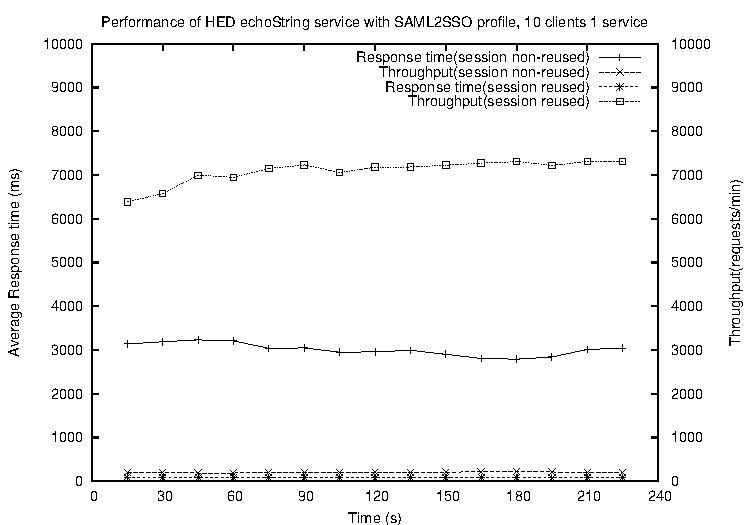
\includegraphics[width=0.9\columnwidth]{SAML2SSO_thread10_nosso.pdf}
\caption{Performance of HED echoString services with SAML2SSO profile: 1 service
and 10 clients; single sign-on is disabled; session used and session not re-used are compared}
\label{fig:SAML2SSO_thread10_nosso}
\end{figure}

\begin{figure}
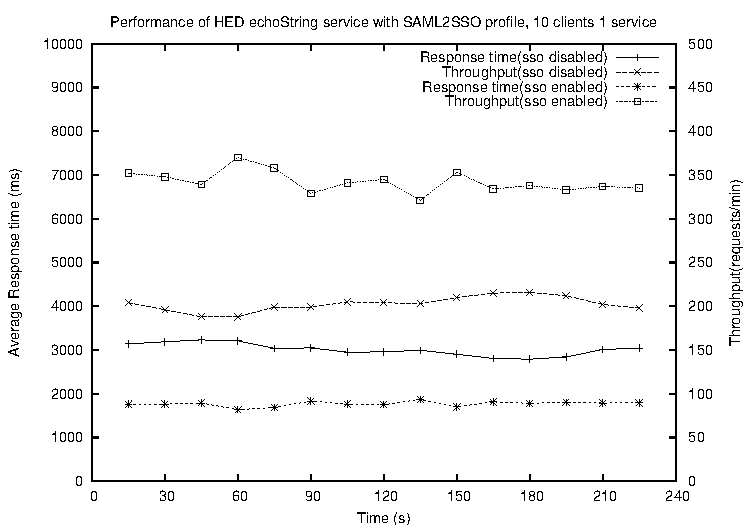
\includegraphics[width=0.9\columnwidth]{SAML2SSO_thread10_nosso_and_sso.pdf}
\caption{Performance of HED echoString services with SAML2SSO profile: 1 service
and 10 clients; session not re-used; single sign-on enabled and single sign-on disabled are compared}
\label{fig:SAML2SSO_thread10_nosso_and_sso}
\end{figure}

\begin{figure}
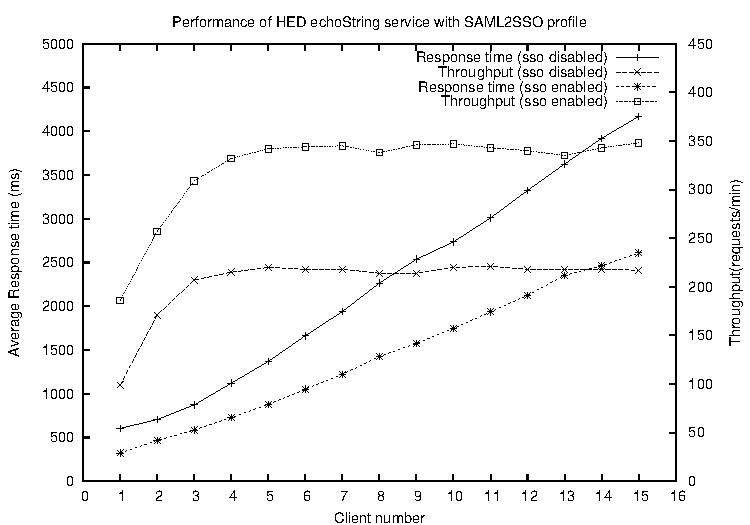
\includegraphics[width=0.9\columnwidth]{SAML2SSO_thread_all.pdf}
\caption{Performance of HED echoString services with SAML2SSO profile:
performance changes with client numbers; session not re-used; single sign-on enabled and 
single sign-on disabled are compared}
\label{fig:SAML2SSO_thread_all}
\end{figure}

We consider two scenarios of authenticating between user agent (client) and IdP: 
SSO enabled, and SSO disabled. ``SSO disabled'' means the successful authentication
session between user agent and IdP is not regarded as valid for the subsequent authentication, and
user is required to authenticate by inputing his username and password on each request.
``SSO enabled'' means the successful authentication session is regarded as valid for the 
subsequent authentication during a short period (we set up this period at 30 minutes).

Since the success of authentication from IdP can be regarded as valid for the whole
session between client and service, we also consider two scenaros in 
usage of the authentication result between client and service: session re-used, and session non-reused.
The client with ``Session reused'' need to accomplish the SAML2SSO
profile only once for all SOAP invocations on this client, while the client with ``Session
non-reused'' will need to accomplish this profile once per SOAP invocation.

Figure~\ref{fig:SAML2SSO_thread10_nosso} shows the average response time and
throughputs for 10 clients running simultaneously against the ``echoString'' service enhanced with SAML2SSO
profile, with single sign-on disabled.

The average response time of ``Session non-reused'' experiments changes little
with the execution duration, and the value is about 3000ms; while the throughput is around 215
requests per minute. Given that the average response time in case of ``Session non-reused'' and
pure SOAP invocation is around 15ms for 10 clients (see Section~\ref{sec:perhedandaxis}),
we can evaluate that the consumption of time for SAML2SSO profile is about 99.5\% of
the whole SOAP invocation with SAML2SSO profile integrated. 

Deeper investigation involving recording the time for each step of SAML2SSO profile
supports the above observation. The average time cost for getting an authentication request
from SP service is about 60ms; the average time cost for authenticating against IdP is about
2750ms; the average time cost for sending the SAML response (from IdP) to SP service is
about 20ms; the average time cost for verifying (by SP service) the signature of SAML
response is around 130ms.

In order to improve the performance of SAML2SSO profile, optimizing the process
between client and IdP is the correct direction, and probably one of the easiest ways is
to enhance the hardware configuration.

One the other hand, the average response time of ``Session reused'' experiments
is about 82 ms, which is almost as short as the value in the pure SOAP invocation experiment in
Section~\ref{sec:perhedandaxis}. The result is reasonable because the time consumption
caused by only once of SAML2SSO execution on one client is relatively small comparing with
the time consumption caused by the following hundreds of pure SOAP invocations on the
same client. So besides improving the performance of SAML2SSO profile, reusing 
the session as long as possbile is also a way to improve the performance of 
Web Service invocation with SAML2SSO profile integrated as authentication approach.

Figure~\ref{fig:SAML2SSO_thread10_nosso_and_sso} depicts performance comparison between single 
sign-on disabled and single sign-on enabled scenarios, for 10 clients running simultaneously 
against the ``echoString'' service enhanced with the SAML2SSO profile, with session not re-used.

The average response time in the ``SSO enabled'' case is about 1700ms, while the throughput is about
340 requests per minutes. The average response time in the ``SSO disabled'' case is about 3000ms, while 
the throughput is about 215 requests per minutes. The comparison shows that the performance 
of ``SSO enabled'' is better than that of ``SSO disabled'', but still on the same quantitative
level.

Figure~\ref{fig:SAML2SSO_thread_all} illustrates performance results for
echoString services that are enhanced with SAML2SSO profile, with client number being changed. In
this set of experiments, the session is not re-used, and single sign-on enabled and single sign-on
disabled scenarios are compared. 

For the situation when single sign-on is disabled, the average response time 
increases linearly with the number of clients, while the throughput increases initially and then 
stays constant (around 215 requests per minute) when the client number is bigger 
than 4. When the client number is 4, the response time is around one second, while the 
throughput of the service is 215 requests per minute, which is almost constant.

For the situation of single sign-on enabled, the average response time 
also increases linearly with the client number, while the throughput also increases initially and then 
saturates at around 340 requests per minute when the client number is bigger 
than 5. When the client number is five, the response time is around 880ms, while the 
throughput of the service is 340 requests per minute, which is almost constant.

We speculate that in order to get acceptable response time, for the case when single sign-on is disabled, 
there should be less than four (including four) concurrent clients if they need to continuously 
participate one SAML2SSO profile; for the case when single sign-on is enabled, 
there should be less than five (including five) concurrent clients if they need to continuously 
participate one SAML2SSO profile.

Given that the throughput of the ``echoString'' service enhanced with mutual
TLS is 13000, and the concurrent client number when throughput reaches saturation is 30, the
performance of ``echoString'' service enhanced with SAML2SSO profile is much worse, both 
with single sign-on disabled and enabled, with the values being 215, 4, and 340, 5, correspondingly.

However, for some typical grid application scenarios, the client normally does
not need to continuously accomplish SAML2SSO profile. For instance, a user could submit a
job which needs a period of time (normally this period is much longer than a few
seconds) to execute, which launches an execution of SAML2SSO profile. 
This user could afterwards query the information as well as the result of
this job, which would launch another execution of SAML2SSO profile. On the other hand,
statistically, users will most probably not access grid system in a concurrent way, rather than in a random way.
Therefore, if we suppose that a user could access grid once per minute, in our test environment, we
can claim that for the case of disabled single sign-on, around 215 clients randomly can be 
supported with acceptable performance, while for the case of single sign-on enabled, around 340 
clients randomly can be supported with acceptable performance.

\subsection{Performance of the SLCS service}
\label{sec:perfslcsserv}

\begin{figure}
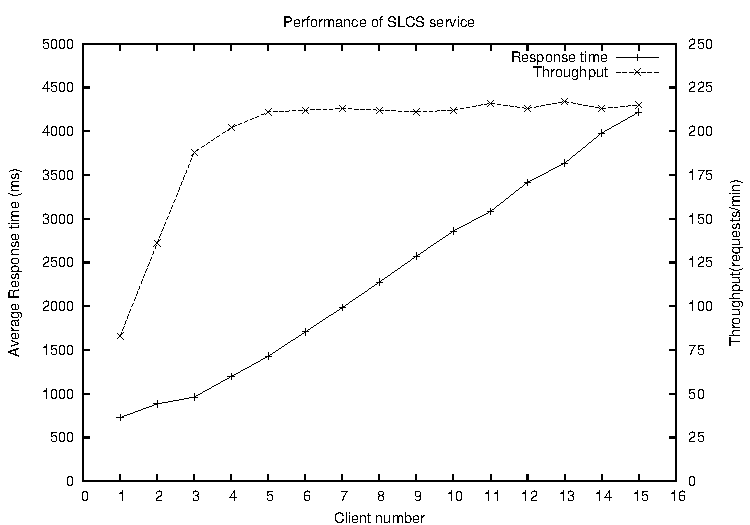
\includegraphics[width=0.9\columnwidth]{SLCS_thread_all.pdf}
\caption{Performance of SLCS service: performance changes with client numbers; single sign-on disabled}
\label{fig:SLCS_thread_all}
\end{figure}

Figure~\ref{fig:SLCS_thread_all} shows performance of the SLCS service.
Since the SLCS is based on the SAML2SSO profile, the response time should be the combination of
time consumption for the SAML2SSO processing and the SLCS processing. In this experiment, SLCS
service and client run on the same set of machine as in Section~\ref{sec:perhedandaxis}. 

Since the time interval of the usage of an SLCS client should be similar to the lifetime of the SLCS
credential, which is 12 hours by default, and the lifetime of a successful authentication session is 
30 minutes by default, enabling single sign-on is not useful in a real deployment because a successful 
authentication session will expire before the next time the SLCS client is used. Therefore, 
we do not enable single sign-on when testing the SLCS service.

The results show that the throughput of SLCS service has the same characteristic
as the throughput of ``echoString'' service enhanced with SAML2SSO profile, with the value being
around 215 requests per minute; and the average response time is close to the value of
``echoString'' service as well, with the value being increased to about 80ms. The increased time
consumption is caused by the creating of X.509 request (1024-bit RSA key pair generation) on the client
side.

Even though the average response time of SLCS service is not very short,
considering the short-lived credential has a relatively long lifetime (12 hours by default) and therefore
client only needs to invoke SLCS service once per 12 hours, the performance is completely acceptable.

\subsection{Performance of the delegation service}
\label{sec:perfdelegserv}

In the last experiment, we evaluate how does the usage of delegation service
affect performance of Web Service invocation. We deployed an ``echoString'' service
plugged with delegation security handler on a machine equipped with 3GHz Intel Pentium dual-core CPU and
2GB memory, Red Hat Enterprise Linux 5, and also configured a client together with delegation
security handler plugged on a machine equipped with 2.0GHz AMD Athlon CPU and 1GB memory, Red Hat
Enterprise Linux 5. Aside from ``echoString'' service and client, a delegation service was deployed on a machine
equipped with 3GHz Intel Pentium dual-core CPU and 2GB memory, Red Hat Enterprise Linux 5.

\begin{figure}
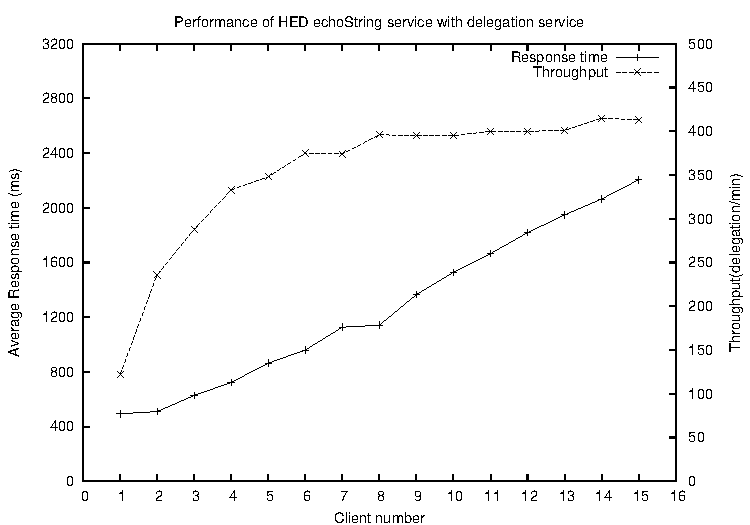
\includegraphics[width=0.9\columnwidth]{Delegation_thread_to_perf.pdf}
\caption{Performance of HED echoString service with credential delegation:
performance changes with the number of clients; echoString service contacts delegation service upon
each service invocation from client}
\label{fig:Delegation_thread_to_perf}
\end{figure}

In this experiment, the client launches a new credential delegation for each
service invocation, and ``echoString'' service acquires delegated credential from delegation service
upon each service invocation.
Figure~\ref{fig:Delegation_thread_to_perf} depicts the average response time and
throughput of the ``echoString'' service with delegation security handler embedded. The
average response time increases linearly with the client number, while the throughput starts to saturate
at around 400 request per minutes when the client number reaches 8.
We conclude that if the client number is bigger than eight, in our test
environment, there is no throughput benefit can be achieved by adding clients.

%-------------------------------------------------------------------------
\section{Related Work}
\label{sec:relatedwork}

There are other efforts that utilize Shibboleth for protecting usage of Grid
resources. The work of Watt and colleagues~\cite{J.Watt06} uses Shibboleth to protect a GridSphere portal and
then indirectly protect Grid services which are deployed in this GridSphere portal.
Another work of Sinott and colleagues~\cite{R.O.Sinnott06} also uses Shibboleth to protect a Grid portal,
moreover, it maintains a few commonly used server certificates which can then be used to access
Grid resources after users have successfully authenticated themselves at a Grid portal
through Shibboleth. Unlike these two solutions that use Shibboleth to protect Grid
portal, the solution in this paper uses Shibboleth or similar standards-based identity federation to
directly protect Grid resource/services, which provides possibility for those Grid applications
that are directly based on Grid interface (e.g., applications that invoke SOAP operations of
remote Grid services), to benefit from identity federation.

GridShib~\cite{T.Scavo07,VWelch05} provides a solution where users can use
X.509 certificates to authenticate to Shibboleth IdP, get back SAML assertion and embed
it in the proxy certificates. The Grid service will then use this SAML assertion for
access control. Unlike the work described in this paper, GridShib still requires users to
possess a X.509 credential, rather than username/password. GridShib also provides another 
solution~\cite{TBarton06} in which a credential service (MyProxy server) is
deployed together with Shibboleth IdP for acting as an online-CA, authenticating the user through
username/password rather than X.509 certificate, and issuing short-lived X.509 credential. The
second solution is similar to the short-lived credential service in our work, while our
solution also provides the option for users to directly authenticate to Grid services via
SAML2.0 SSO profile using their username/password.

Another short-lived credential service is also provided by SWITCH~\cite{switchslcslink}. 
The advantage of our work comparing to the work of SWITCH is that 
our SLCS service is based on the Web Services standard, thus it is easier to
achieve interoperability.

In the aspect of credential delegation, apart from the credential delegation
mechanism of GSI~\cite{IFoster98,VWelch04}, several authors~\cite{MAhsant04} propose a
delegation protocol based on the WS-Trust~\cite{WSTrustlink} to provide a standard and interoperable
protocol for the delegation in Grids. WS-Trust will also be adopted by the ARC middleware
to express the specifications required to define delegation protocol in a standard way.
Gridsite project also implements a X.509 credential delegation solution~\cite{GridSitelink} based on
the Web Service, with which ARC delegation client can be easily made interoperate.

%-------------------------------------------------------------------------
\section{Conclusion And Future Work}
\label{sec:conclusion}
In this paper we propose a Grid single sign-on framework that can utilize
users' federated identity instead of X.509 mutual authentication for authentication,
which we believe can enhance uptake of Grid technlogies by resources owners as well as
by wider range of users.

We implement the SAML2 SSO profile in the ARC Grid middleware, so that the Grid
applications developed by using the application interface provided by this middleware
can easily be adapted to benefit from the federated identity based authentication. 
The performance evaluation shows that even though introduction of SAML2 SSO
profile causes notable performance downgrade, this downgrade can be avoided by reusing the
authentication result for multiple SOAP invocations.
Meanwhile, in order to be compatible with those Grid applications that require
X.509 certificate on the client side, we also implement one Web Service which can be
used for obtaining an X.509 credential based on federated identity, and another Web
Service which can be used for delegating X.509 credential. We believe that the
observed performance is sufficient for creating X.509 certificates and proxy certificates,
considering that the certificates should have a relatively much longer lifetime comparing to the
response time of these two services.
 
Although only the authentication issue has been discussed in this paper, we know that
single sign-in should also include the authorization aspect. The SAML assertion which
includes users' attributes can be used on the service side to achieve attribute-based
authorization. Therefore providing plug-in on the service side to enforce access control using
SAML attribute is considered an important part of the future work.

SimpleSAMLphp~\cite{simplesamllink} provides another implementation of SAML2 SSO
profile, and it has been widely deployed e.g. around Nordic countries for identity federation. Hence
integrating ARC based Grid applications with simpleSAMLphp is considered as another of
future work.



% An example of a floating figure using the graphicx package.
% Note that \label must occur AFTER (or within) \caption.
% For figures, \caption should occur after the \includegraphics.
% Note that IEEEtran v1.7 and later has special internal code that
% is designed to preserve the operation of \label within \caption
% even when the captionsoff option is in effect. However, because
% of issues like this, it may be the safest practice to put all your
% \label just after \caption rather than within \caption{}.
%
% Reminder: the "draftcls" or "draftclsnofoot", not "draft", class
% option should be used if it is desired that the figures are to be
% displayed while in draft mode.
%
%\begin{figure}[!t]
%\centering
%\includegraphics[width=2.5in]{myfigure}
% where an .eps filename suffix will be assumed under latex, 
% and a .pdf suffix will be assumed for pdflatex; or what has been declared
% via \DeclareGraphicsExtensions.
%\caption{Simulation Results}
%\label{fig_sim}
%\end{figure}

% Note that IEEE typically puts floats only at the top, even when this
% results in a large percentage of a column being occupied by floats.


% An example of a double column floating figure using two subfigures.
% (The subfig.sty package must be loaded for this to work.)
% The subfigure \label commands are set within each subfloat command, the
% \label for the overall figure must come after \caption.
% \hfil must be used as a separator to get equal spacing.
% The subfigure.sty package works much the same way, except \subfigure is
% used instead of \subfloat.
%
%\begin{figure*}[!t]
%\centerline{\subfloat[Case I]\includegraphics[width=2.5in]{subfigcase1}%
%\label{fig_first_case}}
%\hfil
%\subfloat[Case II]{\includegraphics[width=2.5in]{subfigcase2}%
%\label{fig_second_case}}}
%\caption{Simulation results}
%\label{fig_sim}
%\end{figure*}
%
% Note that often IEEE papers with subfigures do not employ subfigure
% captions (using the optional argument to \subfloat), but instead will
% reference/describe all of them (a), (b), etc., within the main caption.


% An example of a floating table. Note that, for IEEE style tables, the 
% \caption command should come BEFORE the table. Table text will default to
% \footnotesize as IEEE normally uses this smaller font for tables.
% The \label must come after \caption as always.
%
%\begin{table}[!t]
%% increase table row spacing, adjust to taste
%\renewcommand{\arraystretch}{1.3}
% if using array.sty, it might be a good idea to tweak the value of
% \extrarowheight as needed to properly center the text within the cells
%\caption{An Example of a Table}
%\label{table_example}
%\centering
%% Some packages, such as MDW tools, offer better commands for making tables
%% than the plain LaTeX2e tabular which is used here.
%\begin{tabular}{|c||c|}
%\hline
%One & Two\\
%\hline
%Three & Four\\
%\hline
%\end{tabular}
%\end{table}


\section*{Acknowledgment}
We would thank all of the ARC middleware developers for
their intelligent work. We wish to thank Oxana Smirnova for
vital comments and proof-reading.

% trigger a \newpage just before the given reference
% number - used to balance the columns on the last page
% adjust value as needed - may need to be readjusted if
% the document is modified later
%\IEEEtriggeratref{8}
% The "triggered" command can be changed if desired:
%\IEEEtriggercmd{\enlargethispage{-5in}}

% references section


%\bibliographystyle{IEEEtran}

\begin{thebibliography}{99}

\bibitem{IFoster98}
I. Foster, C. Kesselman, G. Tsudik, and S. Tuecke, A Security Architecture for 
Computational Grids, ACM Conference on Computers and Security, 1998, 83-91.

\bibitem{MEllert07}
M. Ellert et al. Advanced resource connector middleware for lightweight computational 
grids, Future Generation computer systems, 23(2), 219-240 (2007)

\bibitem{KnowARClink}
KnowARC project.  https://www.knowarc.eu/

\bibitem{KnowARCDesignlink}
Design document of new version ARC. https://www.knowarc.eu/documents/Knowarc\_D1.1-1\_07.pdf

\bibitem{WSElink}
Web Services Enhancements 2.0 Service Pack 2. http://msdn.microsoft.com/en-us/library/

\bibitem{A.Shoshan03}
A. Shoshani, A. Sim, and J. Gu, Storage Resource Managers: Essential Components for the Grid, 
Grid Resource Management: State of the Art and Future Trends, Kluwer Publishing, 2003.

\bibitem{Shiblink}
The Shibboleth Project. http://shibboleth.internet2.edu/

\bibitem{SAMLlink}
OASIS Security Assertion Markup Languages (SAML).
www.oasis-open.org/committees/security/

\bibitem{SAMLprofiles}
J. Hughes et al., Profiles for the OASIS Security Assertion Markup
Language (SAML) V2.0, OASIS Standard, 2005

\bibitem{myproxy}
MyProxy Credential Management Service. http://grid.ncsa.uiuc.edu/myproxy/

\bibitem{eduSchemalink}
eduPerson and eduOrg Object shema. http://middleware.internet2.edu/eduperson/

% \bibitem{AlfieriR05}
% R. Alfieri, R. Cecchini, V. Ciaschini, L. dell'Agnello, A. Frohner, K. Lorentey, 
% and F. Spataro. From gridmap-file to voms: managing authorization in a Grid environment. 
% Future Generation Comp. Syst., 21(4), 549-558 (2005)
% 
% \bibitem{RFC3821link}
% RFC 3821- An Internet Attribute Certificate Profile for Authorization. http://www.faqs.org/rfcs/rfc3281.html
% 
% \bibitem{GTlink}
% Globus Toolkit. http://www.globus.org/toolkit/
% 
% \bibitem{gLitelink}
% gLite: lightweight middleware for Grid computing. http://glite.web.cern.ch
% 
% \bibitem{ARClink}
% Advanced Resource Connector. http://www.nordugrid.org/middleware/
% 
% \bibitem{WSSeclink}
% OASIS Web Services Security. www.oasis-open.org/committees/wss/
% 
\bibitem{J.Watt06}
J. Watt, O. Ajayi, J. Jiang, J. Koetsier, R.O. Sinnott. A Shibboleth-Protected 
Privilege Management Infrastructure for e-Science Education. in proceeding of Sixth 
IEEE International Symposium on Cluster Computing and the Grid (CCGRID'06), May 2006,
Singapore.

\bibitem{R.O.Sinnott06}
R.O. Sinnott, J. Jiang, J. Watt, and O. Ajayi. Shibboleth-based access to and 
usage of grid resources. Proceeding of 7th IEEE/ACM International Conference on 
Grid Computing, September 2006, Barcelona.

\bibitem{T.Scavo07}
T. Scavo and V. Welch. A Grid Authorization Model for Science Gateways. International 
Workshop on Grid Computing Environments, 2007.

\bibitem{VWelch05}
V. Welch, T. Barton, K. Keahey and F. Siebenlist. Attributes, Anonymity, and 
Access: Shibboleth and Globus Integration to Facilitate Grid Collaboration. in 
proceeding of 4th Annual PKI R\&D Workshop, 2005.

\bibitem{TBarton06}
T. Barton et al. Identity Federation and Attribute-based Authorization 
through the Globus Toolkit, Shibboleth, Gridshib, and MyProxy. in proceeding 
of 5th Annual PKI R\&D Workshop, 2006.

\bibitem{switchslcslink}
SWITCH Short Lived Credential Service. http://www.switch.ch/Grid/slcs/

\bibitem{VWelch04}
V. Welch et al. X.509 proxy certificate for dynamic delegation. in proceeding 
of the 3rd Annual KI R\&D Workshop, 2004.

\bibitem{MAhsant04}
M. Ahsant, J. Basney, and O. Mulmo. Grid Delegation Protocol. UK Workshop on 
Grid Security Experiences, Oxford. 2004.

\bibitem{WSTrustlink}
OASIS WS-Trust specification. http://docs.oasis-open.org/ws-sx/ws-trust/200512

\bibitem{GridSitelink}
Gridsite delegation service. http://www.gridsite.org/wiki/Delegation\_protocol

\bibitem{simplesamllink}
http://rnd.feide.no/simplesamlphp

\end{thebibliography}

\end{document}
